\documentclass[11pt, oneside]{article} 
\usepackage{geometry}
\geometry{letterpaper} 
\usepackage{graphicx}
	
\usepackage{amssymb}
\usepackage{amsmath}
\usepackage{parskip}
\usepackage{color}
\usepackage{hyperref}

\graphicspath{{/Users/telliott_admin/Tex/png/}}
% \begin{center} 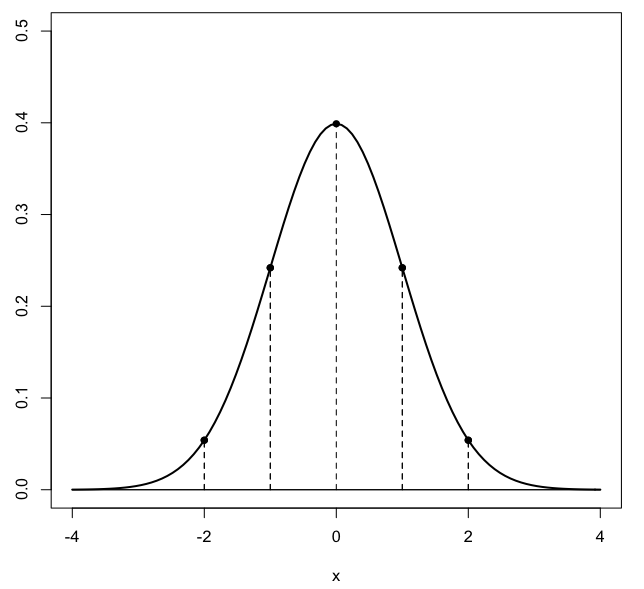
\includegraphics [scale=0.4] {gauss3.png} \end{center}

\title{Ellipse reflected rays}
\date{}

\begin{document}
\maketitle
\Large

In any ellipse, the segments from the foci to any point on the ellipse make equal angles with the tangent.  This means that light rays emitted from one focus and striking anywhere on the ellipse will pass through the other focus upon reflection.  It is the principle behind "whispering galleries."  

Here is a vector proof.  A simple geometric proof follows.

\begin{center} 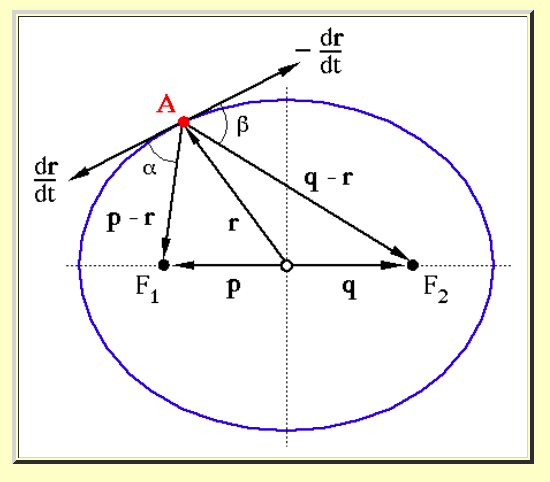
\includegraphics [scale=0.4] {ellipse_reflection.png} \end{center}

\url{http://163.178.103.176/Fisiologia/renal/objetivo_1/Medical_Lithotripsy.htm}

We have seen previously that
\[ \mathbf{r} = \ \langle x,y \rangle \ = \ \langle a \cos t, b \sin t \rangle \ \]
\[ \mathbf{v} = \mathbf{\dot{r}} = \ \langle - a \sin t, b \cos t \rangle \ \]

$\mathbf{v}$ points in the same direction as the tangent.  

Now construct a vector from the origin to the focus $F$ as
\[ \mathbf{q} = \langle c, 0 \rangle \]
and the vector to ${F}'$ is $\mathbf{p}$.

The vector corresponding to $PF$ going toward the focus is
\[ \mathbf{q} - \mathbf{r} \]
(since $\mathbf{r} + PF$ gets to the same place as $\mathbf{q}$).

and the one corresponding to ${PF}'$ is
\[ \mathbf{p} - \mathbf{r} \]

By the standard definition of an ellipse, the sum of the lengths is a constant
\[ | \mathbf{q} - \mathbf{r}| + | \mathbf{p} - \mathbf{r}| = 2a,  \ \ \ \  \text{constant} \]

\subsection*{Lemma about a time-derivative}
$\mathbf{r}$ is a vector function of time.  We need to establish a property of the time-derivative of such a function.  As an example use an arbitrary vector function of time, $\mathbf{w}$.

\[ \frac{d}{dt} |\mathbf{w}| = \frac{d}{dt} \sqrt{\mathbf{w} \cdot \mathbf{w}} \]
by the chain rule:
\[ = \frac{1}{2 \sqrt{\mathbf{w} \cdot \mathbf{w}}} \ \frac{d}{dt} (\mathbf{w} \cdot \mathbf{w}) \]
by the product rule
\[ = \frac{1}{2 \sqrt{\mathbf{w} \cdot \mathbf{w}}} \ (\frac{d \mathbf{w}}{dt} \cdot \mathbf{w} + \mathbf{w} \cdot \frac{d \mathbf{w}}{dt}) \]
\[ = \frac{1}{|\mathbf{w}|} \ (\frac{d \mathbf{w}}{dt} \cdot \mathbf{w}) \]
Hence we have
\[ \frac{d}{dt} |\mathbf{w}| = \frac{d \mathbf{w}}{dt} \cdot \frac{\mathbf{w}}{|\mathbf{w}|} \]

The rate of change of the magnitude of $\mathbf{w}$ is equal to a part of the rate of change of $\mathbf{w}$ itself, namely that part which points in the same direction as $\mathbf{w}$ itself.  Effectively, what we've done is to decompose a differential change in $\mathbf{w}$ with time into two parts, one parallel to $\mathbf{w}$ and one perpendicular to it.  The latter does not contribute to a change in the length.

\subsection*{back to the proof}
We had
\[ | \mathbf{q} - \mathbf{r}| + | \mathbf{p} - \mathbf{r}| = 2a \]
where $2a$ is a constant, so the time-derivative of the left-hand side is also zero.
\[ \frac{d}{dt} \ ( | \mathbf{q} - \mathbf{r}| + | \mathbf{p} - \mathbf{r}| ) = 0 \]

Now using the lemma
\[ \frac{d}{dt} | \mathbf{q} - \mathbf{r}| = \frac{d}{dt} (\mathbf{q} - \mathbf{r}) \cdot \frac{\mathbf{q} - \mathbf{r}}{|\mathbf{q} - \mathbf{r}|} \]
and since $\mathbf{q}$ is constant:
\[ = - \frac{d \mathbf{r}}{dt} \cdot \frac{\mathbf{q} - \mathbf{r}}{|\mathbf{q} - \mathbf{r}|} \]

So for the whole thing we have (rearranging terms):
\[ \frac{d \mathbf{r}}{dt} \cdot \frac{\mathbf{q} - \mathbf{r}}{|\mathbf{q} - \mathbf{r}|} = -\frac{d \mathbf{r}}{dt} \cdot \frac{\mathbf{p} - \mathbf{r}}{|\mathbf{p} - \mathbf{r}|} \]

Take a look at that!
\[ \frac{d \mathbf{r}}{dt} = \mathbf{\dot{r}} = \mathbf{v} \]
so we actually have
\[ \mathbf{v} \cdot \frac{\mathbf{q} - \mathbf{r}}{|\mathbf{q} - \mathbf{r}|} = -\mathbf{v} \cdot \frac{\mathbf{p} - \mathbf{r}}{|\mathbf{p} - \mathbf{r}|} \]

The terms dotted with $\mathbf{v}$ are \emph{unit vectors} from the point to the two foci.

Using the definition of the dot product, for a unit vector $\mathbf{\hat{b}}$
\[ \mathbf{a} \cdot \mathbf{\hat{b}} = |\mathbf{a}| |\mathbf{b}| \cos \theta = |\mathbf{a}| \cos \theta \]

this
\[ \mathbf{v} \cdot \frac{\mathbf{q} - \mathbf{r}}{|\mathbf{q} - \mathbf{r}|} = -\mathbf{v} \cdot \frac{\mathbf{p} - \mathbf{r}}{|\mathbf{p} - \mathbf{r}|} \]
is the same as
\[ |\mathbf{v}| \cos \alpha = |- \mathbf{v}| \cos \beta \]
so
\[ \alpha = \beta \]
$\square$

\subsection*{geometry}
The geometric proof is even simpler.
In another \hyperref[sec:Shortest_path]{\textbf{chapter}}, we considered the problem of the "shortest path."
\begin{center} 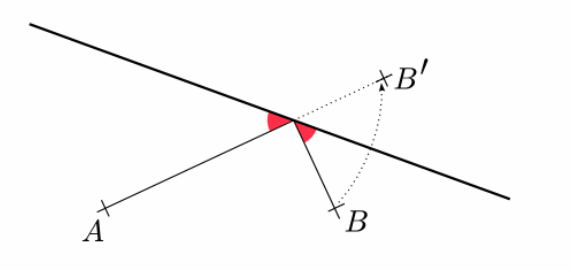
\includegraphics [scale=0.5] {ellipse_reflection2.png} \end{center}

The problem is to go from $A$ to the line and then back to $B$ by the shortest path.  The clever solution is to place $B'$ on the other side of the line at the same distance away.  By definition (see Euclid) the shortest path $A$ to $B'$ is a straight line.

We can use vertical angles (or supplementary angles twice) and then similar triangles to prove that the two angles colored red are equal.

Now consider an enhanced diagram of the same situation:

\begin{center} 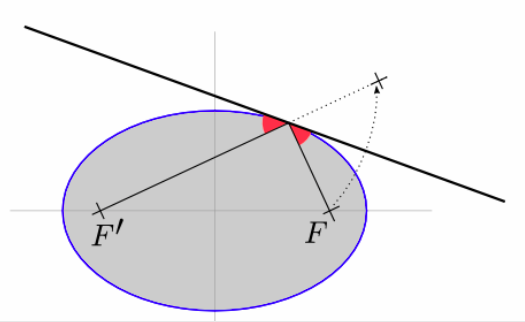
\includegraphics [scale=0.5] {ellipse_reflection3.png} \end{center}
We draw the tangent to the ellipse.  By definition, the tangent has only a single point on the curve.  This point lies at a distance $2a$ from the combined foci.  All other points on the line are farther away from the two foci than the point of intersection.  (You would have to make the string bigger to draw the ellipse that goes through any of those points).

Therefore, the path shown is the shortest path from $F'$ to the tangent and then to $F$.  But we know that for the shortest path the angles colored red are equal.

\url{http://math.stackexchange.com/questions/1063977/how-to-geometrically-prove-the-focal-property-of-ellipse}

\end{document}